\documentclass{standalone}
\usepackage{tikz}
\usepackage{caption}

\definecolor{mycolor0}{RGB}{255,0,0}
\definecolor{mycolor1}{RGB}{0,0,255}
\definecolor{mycolor2}{RGB}{0,0,255}


\begin{document}
	%2D box l =1
	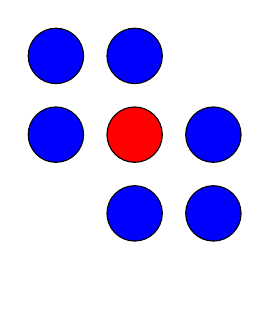
\begin{tikzpicture}[darkstyle/.style={circle,draw,minimum size=20}]
			\foreach \y in {0,...,1}
				\foreach \x in {-1,...,0}
				{
					\pgfmathtruncatemacro{\color}{\x*\x+\y*\y}
					\node[fill=mycolor\color, darkstyle]  at (\x,\y) {}; 
				}
		
			\foreach \y in {0,...,0}
				\foreach \x in {1,...,1}
				{
					\pgfmathtruncatemacro{\color}{\x*\x+\y*\y}
					\node[fill=mycolor\color, darkstyle]  at (\x,\y) {}; 
				}

			\foreach \y in {-1,...,-1}
				\foreach \x in {0,...,1}
				{
					\pgfmathtruncatemacro{\color}{\x*\x+\y*\y}
					\node[fill=mycolor\color, darkstyle]  at (\x,\y) {}; 
				}
				
			\node at (0,-2) {};
	\end{tikzpicture}
\end{document}  